\documentclass[tikz,border=10pt]{standalone}
% Scale: s = 0.015038 cm per px, origin at O
\begin{document}
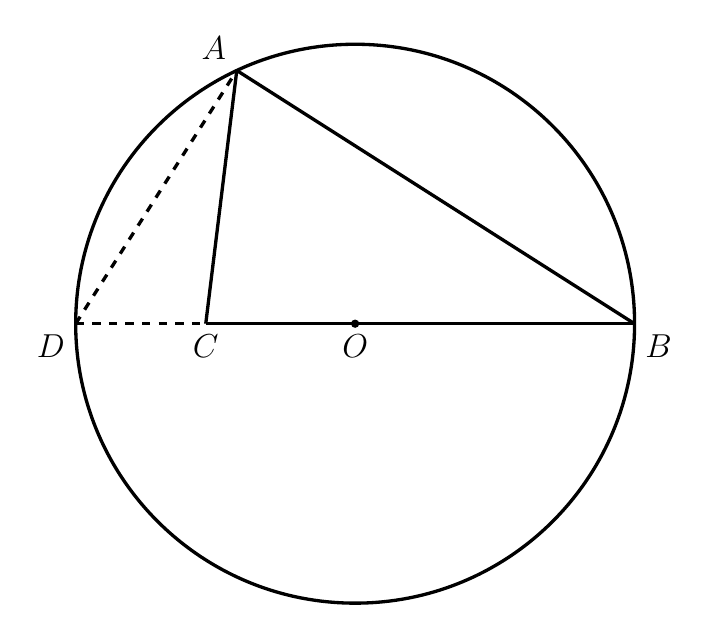
\begin{tikzpicture}[line join=round, line width=1.2pt]
  % Named coordinates (cm)
  \coordinate (O) at (0,0);
  \coordinate (D) at (-3.549,0);
  \coordinate (B) at (3.548,0);
  \coordinate (C) at (-1.897,0);
  \coordinate (A) at (-1.503,3.216);
  \coordinate (X) at (-0.912,0);

  % Circle
  \draw (O) circle (3.549);

  % Centre dot at O
  \fill (O) circle (1.5pt);

  % Diameter: dashed D to X, solid C to B
  \draw[dashed] (D) -- (X);
  \draw (C) -- (B);

  % Segments
  \draw (B) -- (A);
  \draw (A) -- (C);
  \draw[dashed] (D) -- (A);

  % Points and labels
  \node[below left] at (D) {\fontsize{11.5}{13.8}\selectfont $D$};
  \node[below right] at (B) {\fontsize{11.5}{13.8}\selectfont $B$};
  \node[below] at (C) {\fontsize{11.5}{13.8}\selectfont $C$};
  \node[above left] at (A) {\fontsize{11.5}{13.8}\selectfont $A$};
  \node[below] at (O) {\fontsize{11.5}{13.8}\selectfont $O$};
\end{tikzpicture}
\end{document}